\documentclass[11pt,a4paper]{article}

\usepackage[T1]{fontenc}
\usepackage[utf8]{inputenc}
\usepackage{lmodern}
\usepackage[margin=2.5cm]{geometry}
\usepackage{hyperref}
\usepackage{booktabs}
\usepackage{longtable}
\usepackage{array}
\usepackage{ragged2e}
\usepackage{enumitem}

% Wide, ragged columns for env-var tables (single-letter names for \newcolumntype).
\newcolumntype{E}{>{\RaggedRight\arraybackslash}p{6.6cm}}
\newcolumntype{F}{>{\RaggedRight\arraybackslash}p{8.2cm}}
\usepackage{listings}
\usepackage{xcolor}
\usepackage{tikz}
\usetikzlibrary{shapes.geometric, arrows.meta, positioning, calc}

\hypersetup{
  colorlinks=true,
  linkcolor=blue!60!black,
  urlcolor=blue!60!black,
  citecolor=blue!60!black
}

\lstset{
  basicstyle=\ttfamily\small,
  breaklines=true,
  frame=single,
  backgroundcolor=\color{gray!10},
  columns=fullflexible,
  keepspaces=true
}

\title{RAG Chatbot\\[0.5em]\large Technical Documentation}
\author{Author Name}
\date{March 31, 2026}

\begin{document}

\maketitle
\thispagestyle{empty}
\vfill
\begin{center}
\small
This document describes the implementation, technologies, and operation of the RAG Chatbot application: a single-container FastAPI and React stack with Google Gemini and Vertex AI RAG Engine integration.
\end{center}
\vfill
\clearpage

\tableofcontents
\clearpage

%==============================================================================
\section{Introduction}
%==============================================================================

The \textbf{RAG Chatbot} is a full-stack web application that provides a conversational interface similar to modern chat assistants. It combines:

\begin{itemize}[noitemsep]
  \item a \textbf{React} single-page user interface with sidebar, message history, and streaming replies;
  \item a \textbf{FastAPI} backend exposing REST APIs and \textbf{Server-Sent Events (SSE)} for token streaming;
  \item \textbf{Redis} for in-memory persistence of conversations and messages;
  \item \textbf{Google Gemini} (via the \texttt{google-genai} SDK and an API key) for text generation, summarization, and title generation;
  \item \textbf{Vertex AI RAG Engine} for retrieval-augmented generation: relevant chunks are fetched from a configured corpus and injected into the model context.
\end{itemize}

The application is \textbf{publicly accessible}: there is no login or JWT layer. A fixed logical user identifier (\texttt{default}) scopes all Redis data, which keeps the data model ready for future multi-user extensions without changing the API shape.

\textbf{Key features:}
\begin{itemize}[noitemsep]
  \item Conversation list, rename, delete, and new-chat flow.
  \item Streaming assistant responses over SSE without blocking other HTTP requests.
  \item Three-layer \textbf{conversation memory}: running summary of older turns, last 10 messages verbatim, and RAG context for the current query.
  \item Optional static serving of the built React app from the same origin in Docker (empty \texttt{REACT\_APP\_API\_URL} at build time).
\end{itemize}

%==============================================================================
\section{Technology Stack}
%==============================================================================

\subsection{Backend (Python)}

\begin{table}[h]
\centering
\begin{tabular}{@{}llp{7cm}@{}}
\toprule
\textbf{Package} & \textbf{Version} & \textbf{Role} \\
\midrule
FastAPI & 0.115.6 & HTTP API, dependency injection, OpenAPI \\
Uvicorn & 0.34.0 & ASGI server (with standard extras) \\
redis[hiredis] & 5.2.1 & Async Redis client and C parser \\
Pydantic & 2.10.4 & Request/response validation \\
pydantic-settings & 2.7.1 & Environment-based configuration \\
google-genai & $\geq$1.0.0 & Gemini client (generate, stream) \\
google-auth & $\geq$2.20.0 & Service account OAuth2 for Vertex REST \\
httpx & $\geq$0.27.0 & Async HTTP client for RAG REST calls \\
\bottomrule
\end{tabular}
\caption{Backend Python dependencies (from \texttt{requirements.txt}).}
\end{table}

\subsection{Frontend (Node.js / React)}

\begin{table}[h]
\centering
\begin{tabular}{@{}llp{6.5cm}@{}}
\toprule
\textbf{Package} & \textbf{Version} & \textbf{Role} \\
\midrule
react / react-dom & 18.3.x & UI framework \\
react-scripts & 5.0.1 & Create React App build toolchain \\
react-markdown & 9.x & Markdown rendering in messages \\
remark-gfm & 4.x & GitHub-flavored Markdown \\
react-syntax-highlighter & 15.x & Code block highlighting (Prism) \\
react-icons & 5.x & Icon set for sidebar and controls \\
\bottomrule
\end{tabular}
\caption{Frontend dependencies (from \texttt{package.json}).}
\end{table}

\subsection{Infrastructure and runtime}

\begin{itemize}[noitemsep]
  \item \textbf{Docker}: multi-stage image --- Node 22 Alpine builds the frontend; Python 3.13 Alpine runs the API, embedded Redis, and Uvicorn.
  \item \textbf{Docker Compose}: single service \texttt{chatbot}, port mapping, environment variables, optional read-only mount for GCP service account JSON.
  \item \textbf{Redis}: runs inside the container in production (\texttt{redis-server --daemonize yes}) with persistence disabled for simplicity (\texttt{--save "" --appendonly no}).
\end{itemize}

\subsection{AI and Google Cloud}

\begin{itemize}[noitemsep]
  \item \textbf{Gemini model} (configurable, default \texttt{gemini-2.5-flash}): chat completion, streaming, summarization, conversation titles.
  \item \textbf{Vertex AI RAG}: \texttt{retrieveContexts} REST API (\texttt{v1beta1}) against \texttt{RAG\_CORPUS\_NAME}, authenticated with a \textbf{service account} access token (not the Gemini API key).
\end{itemize}

%==============================================================================
\section{System Architecture}
%==============================================================================

\subsection{High-level view}

Figure~\ref{fig:arch} shows the main components and data flows.

\begin{figure}[htbp]
\centering
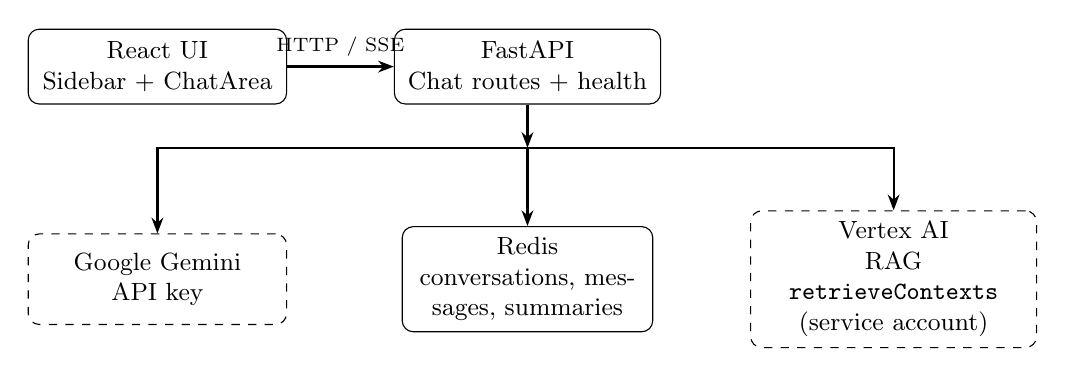
\begin{tikzpicture}[
  box/.style={rectangle, draw, rounded corners, minimum height=0.95cm, align=center, font=\small, inner sep=4pt},
  cloud/.style={rectangle, draw, dashed, rounded corners, minimum height=1.15cm, align=center, font=\small, inner sep=4pt},
  arrow/.style={-{Stealth[length=2mm]}, thick}
]
% Explicit coordinates avoid overlap between Redis (under API) and the cloud nodes.
\node[box, text width=3.0cm] (ui) at (0,0) {React UI\\Sidebar + ChatArea};
\node[box, text width=3.1cm] (api) at (4.7,0) {FastAPI\\Chat routes + health};
\draw[arrow] (ui.east) -- node[above, font=\scriptsize] {HTTP / SSE} (api.west);

\node[box, text width=2.9cm] (redis) at (4.7,-2.7) {Redis\\conversations, messages, summaries};
\node[cloud, text width=3.0cm] (gemini) at (0,-2.7) {Google Gemini\\API key};
\node[cloud, text width=3.35cm] (vertex) at (9.35,-2.7) {Vertex AI\\RAG \texttt{retrieveContexts}\\(service account)};

% Junction below API: vertical stem, then Redis + branches to Gemini and Vertex.
\coordinate (hub) at ($(api.south)+(0,-0.55)$);
\draw[arrow] (api.south) -- (hub);
\draw[arrow] (hub) -- (redis.north);
\draw[arrow] (hub) -| (gemini.north);
\draw[arrow] (hub) -| (vertex.north);

\end{tikzpicture}
\caption{Logical architecture: browser, API, Redis, and external AI services.}
\label{fig:arch}
\end{figure}

\subsection{Responsibilities}

\begin{description}[style=nextline, font=\normalfont\bfseries]
  \item[React frontend] Renders the chat layout, loads conversations and messages, sends user input to \texttt{POST /api/chat/send}, parses SSE lines for chunks and final \texttt{conversation\_id}.
  \item[FastAPI backend] Validates requests, reads/writes Redis, orchestrates summarization and RAG retrieval, streams Gemini output as SSE events.
  \item[Redis] Stores conversation metadata (hash + sorted set index), message lists (JSON per element), per-conversation message ID counter, and optional running summary string.
  \item[Gemini] Produces assistant text (streaming), incremental conversation summaries, and short titles for new threads.
  \item[Vertex RAG] Returns ranked text chunks for the user query; the backend concatenates them into a single context block for the model.
\end{description}

%==============================================================================
\section{Backend Implementation}
%==============================================================================

\subsection{Project structure}

\begin{lstlisting}
backend/
  requirements.txt
  app/
    main.py              # FastAPI app, CORS, lifespan, static SPA
    core/
      config.py          # Settings from environment
      database.py        # Redis pool init/close/get
    models/
      chat.py            # Pydantic schemas + Conversations/Messages tables
    routes/
      chat.py            # REST + SSE send endpoint
    services/
      rag_service.py     # Gemini, RAG REST, summarization, streaming
\end{lstlisting}

\subsection{Configuration (\texttt{core/config.py})}

Settings are loaded with \textbf{pydantic-settings} from environment variables and optional \texttt{.env}. Relevant fields:

\begin{itemize}[noitemsep]
  \item \texttt{REDIS\_URL} --- Redis connection string.
  \item \texttt{GCP\_PROJECT\_ID}, \texttt{GCP\_LOCATION}, \texttt{RAG\_CORPUS\_NAME} --- Vertex RAG corpus resource name and routing.
  \item \texttt{GEMINI\_MODEL\_NAME} --- Model id for generation.
  \item \texttt{GOOGLE\_API\_KEY} --- Gemini API authentication.
  \item \texttt{GOOGLE\_APPLICATION\_CREDENTIALS} --- Path to service account JSON for RAG REST calls.
  \item \texttt{CORS\_ORIGINS} --- Comma-separated list or \texttt{*}.
  \item \texttt{STATIC\_DIR} --- If set, enables mounting built React assets and SPA fallback routes.
\end{itemize}

\texttt{get\_settings()} is cached with \texttt{lru\_cache} for a single process lifetime.

\subsection{Database layer (\texttt{core/database.py})}

\texttt{init\_redis()} creates an async Redis client from \texttt{settings.REDIS\_URL} with \texttt{decode\_responses=True} and pings the server. \texttt{get\_redis()} returns the global pool used by routes. \texttt{close\_redis()} closes the connection on application shutdown (FastAPI lifespan).

\subsection{Data models (\texttt{models/chat.py})}

\textbf{Pydantic models} define API contracts: \texttt{ConversationCreate}, \texttt{ConversationUpdate}, \texttt{ConversationResponse}, \texttt{MessageResponse}, \texttt{ChatRequest}.

\textbf{Redis key schema:}
\begin{itemize}[noitemsep]
  \item \texttt{conv:\{id\}} --- hash: \texttt{id}, \texttt{user\_id}, \texttt{title}, \texttt{model}, \texttt{system\_prompt}, \texttt{created\_at}, \texttt{updated\_at}.
  \item \texttt{user\_convs:\{user\_id\}} --- sorted set: member conversation id, score = last update timestamp (for ordering).
  \item \texttt{msgs:\{conv\_id\}} --- list of JSON-serialized message objects (oldest first).
  \item \texttt{msg\_counter:\{conv\_id\}} --- integer string for monotonic message ids.
  \item \texttt{conv\_summary:\{conv\_id\}} --- string: running summary for context compression.
\end{itemize}

\textbf{Table-class pattern:} \texttt{ConversationsTable} and \texttt{MessagesTable} encapsulate Redis commands (mirroring a thin ORM layer), keeping route handlers declarative. Singleton instances \texttt{Conversations} and \texttt{Messages} are imported by routes.

\subsection{API routes (\texttt{routes/chat.py})}

\begin{itemize}[noitemsep]
  \item \texttt{DEFAULT\_USER = "default"} for all ownership checks.
  \item CRUD for conversations and listing messages under \texttt{/api/chat/...}.
  \item \texttt{POST /api/chat/send}: resolves or creates a conversation, appends the user message, optionally refreshes the summary, calls \texttt{retrieve\_rag\_context}, builds \texttt{context\_messages}, streams SSE from \texttt{generate\_streaming\_response}, persists the assistant message, and may generate a title for brand-new threads. A final SSE event carries \texttt{conversation\_id}.
\end{itemize}

Streaming uses an async generator that forwards chunks from the RAG service and collects the full assistant text in a \texttt{result\_holder} list for persistence after the stream completes (avoiding re-parsing every SSE payload).

\subsection{RAG service (\texttt{services/rag\_service.py})}

\begin{itemize}[noitemsep]
  \item \textbf{Initialization:} Lazy singleton Gemini client from \texttt{GOOGLE\_API\_KEY}; optional service account credentials for Vertex.
  \item \textbf{\texttt{retrieve\_rag\_context(query)}:} POST to\\
  \texttt{https://\{location\}-aiplatform.googleapis.com/v1beta1/projects/\{project\}/locations/\{location\}:retrieveContexts}\\
  with JSON body containing \texttt{vertex\_rag\_store} and \texttt{query} (text, top-k, optional distance filter). Parses \texttt{contexts} into a single string with source URIs when present.
  \item \textbf{\texttt{summarize\_messages}:} Calls Gemini with a fixed summarizer prompt; supports folding in a previous summary.
  \item \textbf{\texttt{build\_context\_messages}:} Prepends system prompt, optional summary block, optional RAG block, then maps recent Redis messages to alternating user/model roles for the Gemini \texttt{contents} API.
  \item \textbf{\texttt{generate\_streaming\_response}:} Wraps synchronous streaming in \texttt{run\_in\_executor}, yields \texttt{data: \{json\}\\n\\n} SSE lines and appends full text to \texttt{result\_holder}.
  \item \textbf{\texttt{generate\_title\_for\_conversation}:} Short title from first user message; uses \texttt{(resp.text or "").strip()} to tolerate empty API responses.
\end{itemize}

%==============================================================================
\section{Frontend Implementation}
%==============================================================================

\subsection{Project structure}

\begin{lstlisting}
frontend/
  public/index.html
  src/
    index.js, index.css
    App.js, App.css
    components/
      Sidebar.js, Sidebar.css
      ChatArea.js, ChatArea.css
    services/
      api.js
\end{lstlisting}

Empty directories \texttt{context/} and \texttt{pages/} may exist from earlier scaffolding and are unused.

\subsection{Entry and app shell (\texttt{App.js})}

\texttt{App} holds state: conversation list, active conversation id, messages, streaming buffer, streaming flag, sidebar collapse. Effects load conversations on mount and reload messages when \texttt{activeId} changes. \texttt{sendMessageStream} receives chunks into a ref-backed buffer; on completion the assistant message is appended and the sidebar refreshes. Stopping generation clears streaming state and appends partial text with a stopped marker.

\subsection{Components}

\textbf{Sidebar:} Lists conversations (buttons for accessibility), search filter, new chat, collapse toggle, rename and delete actions calling REST helpers.

\textbf{ChatArea:} Empty state with suggested prompts; message list with \texttt{ReactMarkdown} and \texttt{remark-gfm}; code blocks via \texttt{react-syntax-highlighter} (Prism, oneDark); typing indicator while streaming with no tokens yet; auto-growing textarea; send vs stop button.

\subsection{API layer (\texttt{services/api.js})}

\texttt{request()} wraps \texttt{fetch} with JSON and error handling. Exported functions: \texttt{getConversations}, \texttt{updateConversation}, \texttt{deleteConversation}, \texttt{getMessages}, \texttt{sendMessageStream}. The stream reader decodes lines starting with \texttt{data: }, parses JSON, dispatches \texttt{onChunk} for content deltas, collects errors and final \texttt{conversation\_id}, then invokes \texttt{onError} and/or \texttt{onDone} after the stream ends.

\texttt{REACT\_APP\_API\_URL} defaults to empty string for same-origin deployment; local dev sets \texttt{http://localhost:8000}.

%==============================================================================
\section{Conversation Memory Strategy}
%==============================================================================

For each \texttt{POST /api/chat/send}, the backend builds context as follows:

\begin{enumerate}[noitemsep]
  \item \textbf{Running summary} --- Stored in Redis at \texttt{conv\_summary:\{id\}}. When the total message count exceeds 10 and either no summary exists yet or the count is a multiple of 4, older messages (everything except the last 10) are sent to \texttt{summarize\_messages} together with the prior summary; the result is written back to Redis.
  \item \textbf{Recent window} --- The last 10 messages (including the new user turn) are passed verbatim as chat history to Gemini.
  \item \textbf{RAG context} --- \texttt{retrieve\_rag\_context} uses the current user message text as the query; retrieved chunks are injected as a labeled block in \texttt{build\_context\_messages}.
\end{enumerate}

This limits token growth on long threads while preserving salient facts in the summary and fresh detail in the last turns.

%==============================================================================
\section{RAG Integration}
%==============================================================================

\begin{itemize}[noitemsep]
  \item \textbf{Gemini:} Authenticated with \texttt{GOOGLE\_API\_KEY} through \texttt{google.genai.Client}.
  \item \textbf{Vertex RAG:} Requires \texttt{GOOGLE\_APPLICATION\_CREDENTIALS} pointing to a JSON key with permission to call Vertex AI in the project/region. The code exchanges credentials for an OAuth2 access token (with short-lived caching) and sends it in the \texttt{Authorization: Bearer} header.
  \item If the corpus or credentials are missing, RAG retrieval returns \texttt{None} and the model still answers using system prompt, summary, and recent messages only.
  \item Chunking and embedding are managed inside the RAG corpus (e.g.\ managed vector store in GCP); this application only queries the corpus by text.
\end{itemize}

%==============================================================================
\section{Deployment}
%==============================================================================

\subsection{Dockerfile (multi-stage)}

\textbf{Stage 1 (\texttt{frontend-build}):} \texttt{node:22-alpine}, \texttt{npm install}, copy sources, \texttt{ENV REACT\_APP\_API\_URL=""}, \texttt{npm run build} $\rightarrow$ static files under \texttt{/build/build}.

\textbf{Stage 2 (runtime):} \texttt{python:3.13-alpine}, install \texttt{gcc}, \texttt{musl-dev}, \texttt{libffi-dev}, \texttt{redis}; \texttt{pip install -r requirements.txt}; copy backend; copy frontend build to \texttt{/app/static}; set \texttt{STATIC\_DIR} and \texttt{REDIS\_URL}; \texttt{start.sh} runs \texttt{redis-server} daemonized then \texttt{uvicorn app.main:app --host 0.0.0.0 --port 8000}.

\subsection{Docker Compose}

Service \texttt{chatbot}, build context project root, container name \texttt{rag-chatbot}, port \texttt{\$\{PORT:-8000\}:8000}, environment variables for Redis, GCP, Gemini, CORS, static dir, volume\\
\texttt{\$\{GCP\_SA\_KEY\_PATH:-/dev/null\}:/app/credentials/sa-key.json:ro}.

\subsection{Environment variables (reference)}

\begin{longtable}{@{}E F@{}}
\toprule
\textbf{Variable} & \textbf{Description} \\
\midrule
\endhead
\ttfamily\footnotesize REDIS\_URL\normalfont\normalsize & Redis URL (container: \texttt{redis://localhost:6379/0}). \\
\ttfamily\footnotesize GCP\_PROJECT\_ID\normalfont\normalsize & Google Cloud project id. \\
\ttfamily\footnotesize GCP\_LOCATION\normalfont\normalsize & Vertex region (e.g.\ \texttt{europe-west3}). \\
\ttfamily\footnotesize RAG\_CORPUS\_NAME\normalfont\normalsize & Full resource name of the RAG corpus. \\
\ttfamily\footnotesize GEMINI\_MODEL\_NAME\normalfont\normalsize & Gemini model id. \\
\ttfamily\footnotesize GOOGLE\_API\_KEY\normalfont\normalsize & API key for Gemini (Generative Language API). \\
\ttfamily\footnotesize GOOGLE\_APPLICATION\_\allowbreak CREDENTIALS\normalfont\normalsize & Filesystem path to service account JSON inside the container (e.g.\ \texttt{/app/credentials/sa-key.json}). \\
\ttfamily\footnotesize CORS\_ORIGINS\normalfont\normalsize & Allowed origins (comma-separated) or \texttt{*}. \\
\ttfamily\footnotesize STATIC\_DIR\normalfont\normalsize & Path to built SPA (\texttt{/app/static} in Docker). \\
\ttfamily\footnotesize PORT\normalfont\normalsize & Host port for Compose (optional, default 8000). \\
\ttfamily\footnotesize GCP\_SA\_KEY\_PATH\normalfont\normalsize & Host path to key file mounted read-only at \texttt{/app/credentials/sa-key.json}. \\
\bottomrule
\end{longtable}

%==============================================================================
\section{API Reference}
%==============================================================================

\begin{longtable}{@{}llp{6.8cm}@{}}
\toprule
\textbf{Method} & \textbf{Path} & \textbf{Description} \\
\midrule
\endhead
GET & \texttt{/api/health} & Health check; returns \texttt{\{"status": "ok"\}}. \\
GET & \texttt{/api/chat/conversations} & List all conversations (default user). \\
POST & \texttt{/api/chat/conversations} & Create a conversation (optional; UI creates via send). \\
GET & \texttt{/api/chat/conversations/\{id\}} & Get one conversation metadata. \\
PUT & \texttt{/api/chat/conversations/\{id\}} & Update title, model, or system prompt fields. \\
DELETE & \texttt{/api/chat/conversations/\{id\}} & Delete conversation and related Redis keys. \\
GET & \texttt{/api/chat/conversations/\{id\}/messages} & List messages in order. \\
POST & \texttt{/api/chat/send} & Body: \texttt{\{ "message": string, "conversation\_id": string|null \}}. Response: \texttt{text/event-stream} SSE (content chunks, then \texttt{conversation\_id}). \\
\bottomrule
\end{longtable}

\noindent\textbf{SSE payload shapes (JSON after \texttt{data: }):}
\begin{itemize}[noitemsep]
  \item Streaming chunk: \texttt{\{"content": "<delta>", "done": false\}}
  \item Stream finished: \texttt{\{"content": "", "done": true\}}
  \item Error: \texttt{\{"error": "<message>"\}}
  \item Final: \texttt{\{"conversation\_id": "<uuid>"\}}
\end{itemize}
Line \texttt{data: [DONE]} may appear after completion.

\end{document}
